\section{Les différentes machines}

\subsection{Plateformes de force}

Ces plateformes mesurent les forces appliquées par les pieds sur leur surface grâce à des capteurs, basés sur des jauges de contrainte ou des capteurs piézoélectriques. 
Ces capteurs enregistrent les composantes des forces dans les trois axes (X, Y, Z) et les moments de force autour de ces axes. 
Les données relevées permettent de calculer le \textbf{Centre de Pression (CdP)}, reflétant la répartition du poids et des ajustements posturaux du corps. 
Le CdP est alors suivi en temps réel dans le but d'analyser les oscillations posturales.

Elles sont fréquemment utilisées pour évaluer l’équilibre postural, la répartition du poids ainsi que les ajustements dynamiques du corps. 
Elles sont essentielles dans des domaines comme la neurologie (troubles de l’équilibre), la rééducation (suivi de récupération post-blessure), et le sport (analyse de la performance ou de l’impact). 
Ces dispositifs contribuent également à identifier les asymétries et à évaluer le risque de chute chez les personnes âgées.

\subsubsection{Exemples (liens) :}
\begin{itemize}
  \item \href{https://www.amti.biz/product-line/force-plates/}{\textbf{AMTI AccuSway Plus}}
  \item \href{https://www.bertec.com/products/force-plates}{\textbf{Bertec Force Plate}}
\end{itemize}

\begin{figure}[ht]
  \centering
  \begin{subfigure}[b]{0.45\textwidth}
    \centering
    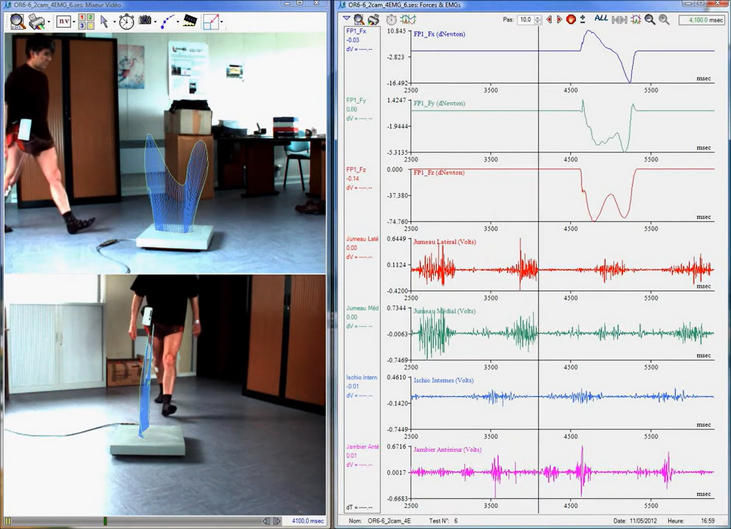
\includegraphics[height=5cm]{images/OR6.png}
    \caption{Logiciel OR6}\label{fig:OR6}
  \end{subfigure}
  \begin{subfigure}[b]{0.45\textwidth}
    \centering
    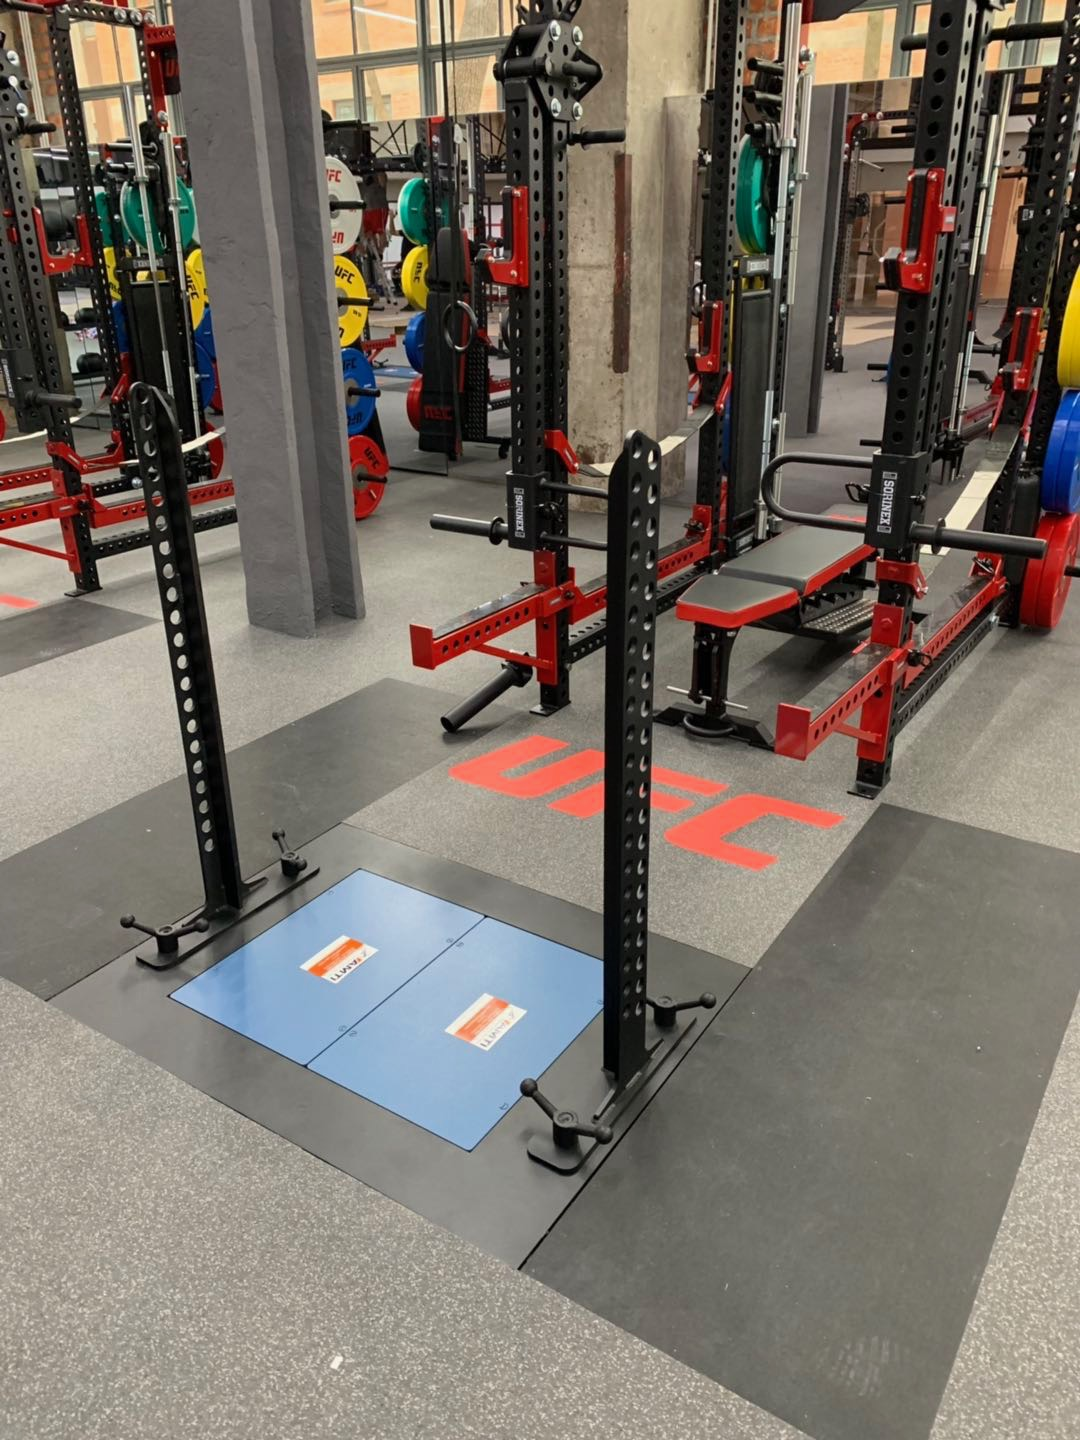
\includegraphics[height=5cm]{images/AMTI.jpeg}
    \caption{Plateforme de force (UFC)}\label{fig:AMTI}
  \end{subfigure}
  \caption{Illustration d'un logiciel et d'une plateforme de force}\label{fig:exemple_plateforme_force}
\end{figure}


\subsection{Centrales inertielles (IMU)}

Des capteurs tels que les accéléromètres, les gyroscopes et parfois les magnétomètres sont employés dans les centrales inertielles pour quantifier les mouvements corporels. 
Les accélérations linéaires sont détectées par l'accéléromètre sur les axes X, Y et Z, tandis que le gyroscope évalue les vitesses angulaires autour de ces axes. 
Lorsqu'il est intégré, le magnétomètre donne une direction absolue par rapport au champ magnétique de la Terre. 
Ces détecteurs facilitent le suivi de la position, de l'orientation et des trajets des segments du corps, y compris dans des contextes mobiles.

Les IMU sont utilisées pour l’analyse de la posture et des mouvements dans des environnements dynamiques, en dehors des laboratoires.
En sport, elles aident à optimiser les performances en analysant les mouvements des athlètes. 
En rééducation, elles permettent de suivre les progrès des patients dans leurs activités quotidiennes. 
Ces dispositifs sont également courants dans les études biomécaniques pour évaluer la stabilité dynamique et les stratégies d’équilibre.

\subsubsection{Exemples :}
\begin{itemize}
  \item \href{https://www.movella.com/products/wearables/xsens-mtw-awinda}{\textbf{Xsens MTw Awinda}}
  \item \href{https://www.noraxon.com/products/myomotion/}{\textbf{Noraxon MyoMotion}}
\end{itemize}

\begin{figure}[ht]
  \centering
  \begin{subfigure}[b]{0.45\textwidth}
    \centering
    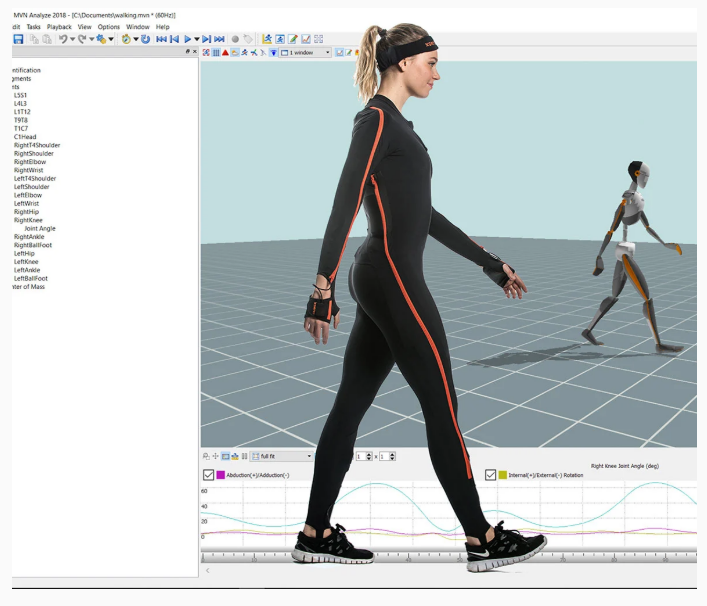
\includegraphics[height=5cm]{images/xsens.png}
    \caption{Logiciel MVN Analyse}\label{fig:mvn_analyse}
  \end{subfigure}
  \begin{subfigure}[b]{0.45\textwidth}
    \centering
    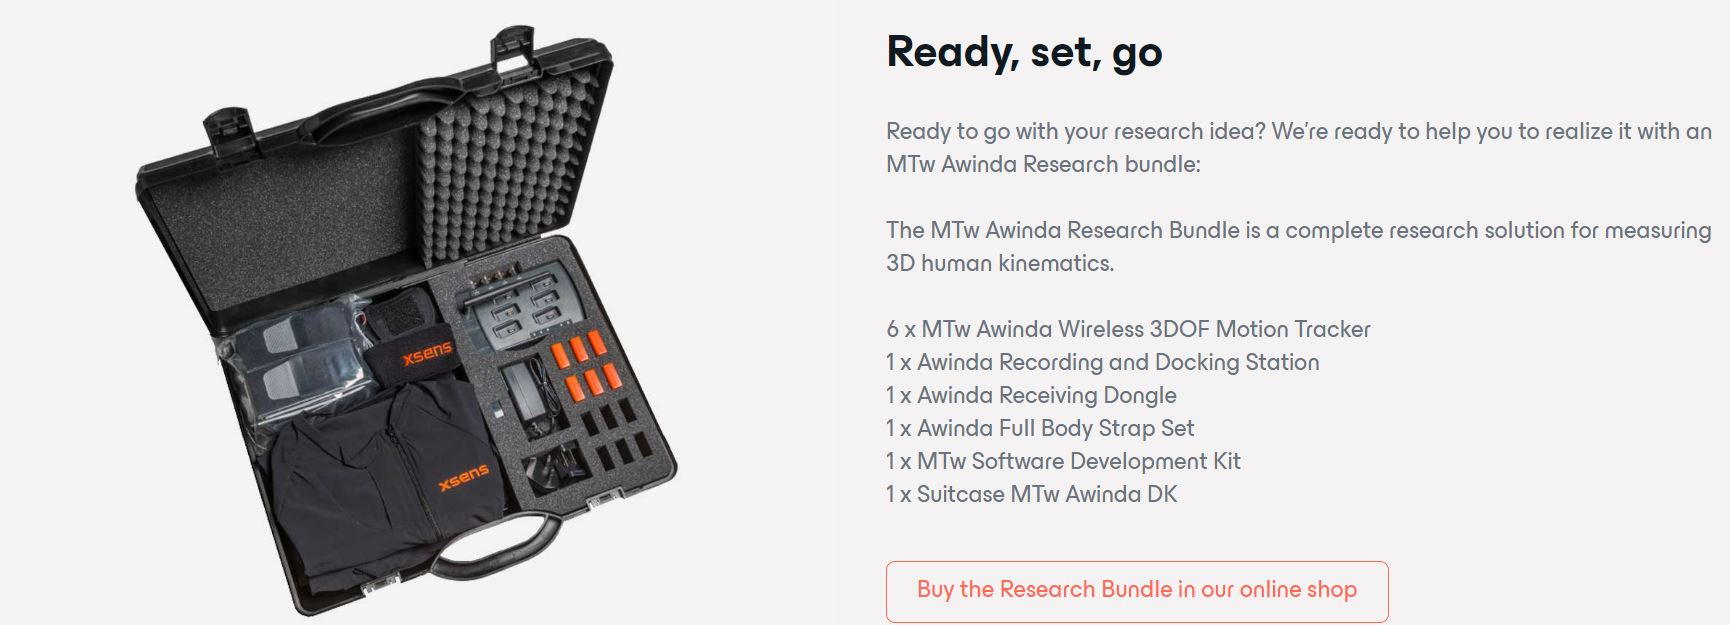
\includegraphics[height=5cm, width=\textwidth]{images/mtw_awinda.jpg}
    \caption{MTw Awinda Research bundle}\label{fig:MTw_awinda_research}
  \end{subfigure}
  \caption{Exemple de matériel utilisé dans le cadre des mesures inertielles}\label{fig:exemple_mesures_inertielles}
\end{figure}

\subsection{Plateformes stabilométriques}

Les plateformes stabilométriques, à l'instar des plateformes de force, mettent particulièrement l'accent sur l'étude des mouvements posturaux en évaluant les forces verticales et les déplacements dans les plans horizontal et vertical.
Ces plateformes disposent fréquemment d'instruments additionnels, tels que des surfaces instables ou des systèmes de visualisation interactifs, pour perturber l'équilibre et examiner les réactions compensatoires du patient.

Ces dispositifs sont utilisés pour évaluer la stabilité posturale en position debout, notamment chez des patients atteints de troubles neurologiques ou vestibulaires.
Ils sont également utilisés pour détecter les déficiences proprioceptives et pour la rééducation.
En gériatrie, ils permettent d’évaluer les risques de chute, et en sport, ils servent à optimiser les stratégies d’équilibre.

\subsubsection{Exemples : }
\begin{itemize}
  \item \href{https://www.stabilometry.com/}{\textbf{Stabilo Stabilometric Platform}}
  \item \href{https://www.natus.com/products/balancemaster}{\textbf{BalanceMaster}}
\end{itemize}


\begin{figure}[H]
  \centering
  \begin{subfigure}[b]{0.45\textwidth}
    \centering
    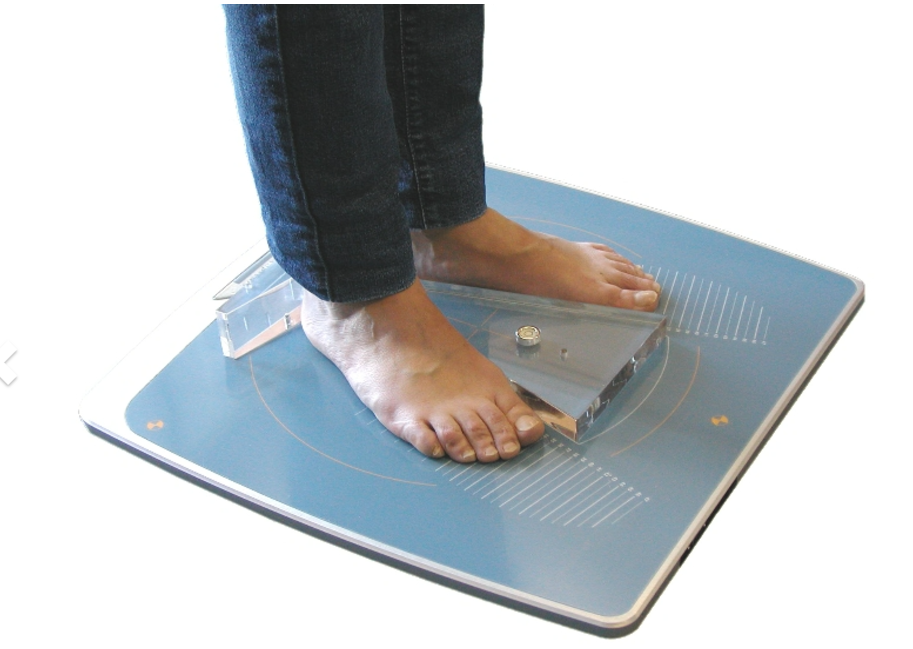
\includegraphics[height=5cm]{images/plateforme-stabilometrique.png}
    \caption{Plateforme stabilométrique}\label{fig:plateforme_stabilometrique}
  \end{subfigure}
  \begin{subfigure}[b]{0.45\textwidth}
    \centering
    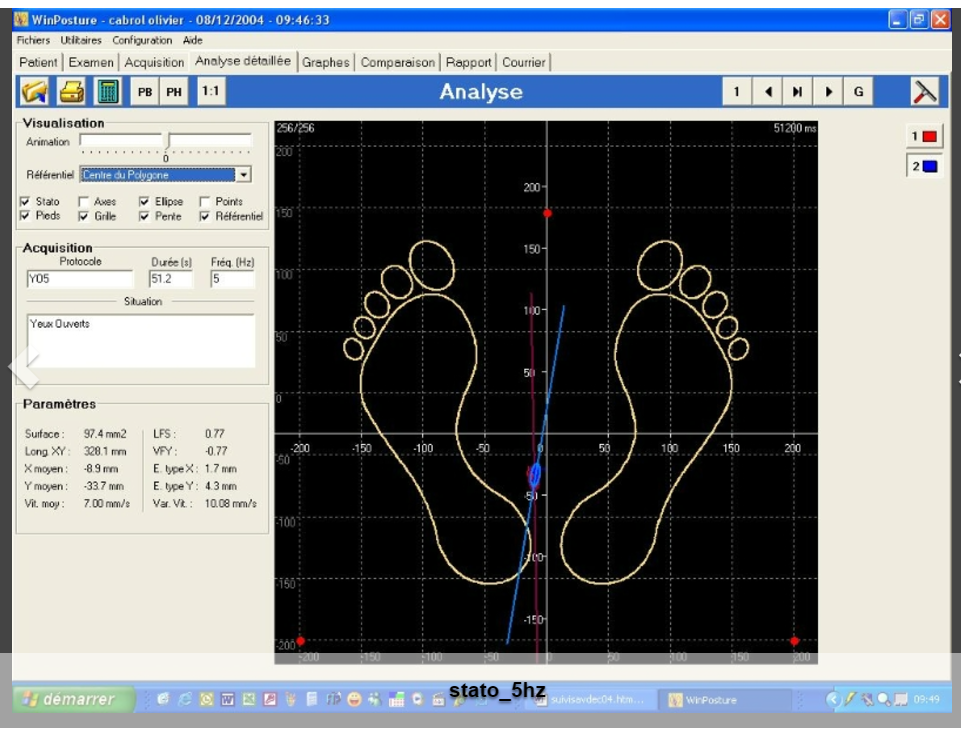
\includegraphics[height=5cm]{images/winposture}
    \caption{Logiciel Winposture}\label{fig:winposture}
  \end{subfigure}
  \begin{subfigure}[b]{0.45\textwidth}
    \centering
    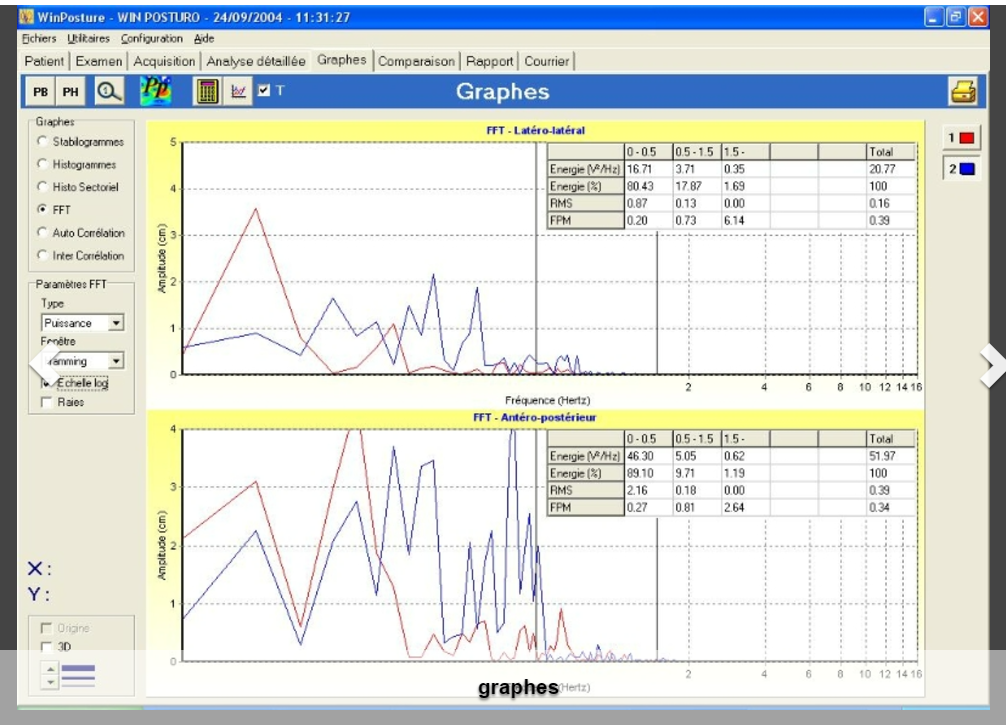
\includegraphics[height=5cm, width=\textwidth]{images/winposture-graph.png}
    \caption{Graphiques logiciel Winposture}\label{fig:winposture_graph}
  \end{subfigure}
  \caption{Exemple de dispositifs stabilométriques}\label{fig:exemple_posturographie}
\end{figure}

\subsection{Plateformes de posturographie}

Les dispositifs de posturographie évaluent les forces verticales que les pieds exercent pour déterminer les coordonnées du Centre de Pression (CdP).
Certaines plateformes intègrent des fonctionnalités dynamiques, telles que des surfaces en mouvement ou en inclinaison, afin de reproduire des perturbations de l'équilibre.

Ces plateformes servent à l'évaluation clinique de la posture, notamment dans des secteurs comme la neurologie (compréhension des troubles de l'équilibre et des affections vestibulaires), la gériatrie (pour prévenir les chutes) et la réhabilitation suite à des blessures ou interventions chirurgicales. Elles sont aussi fréquemment employées dans des recherches sur l'équilibre.

\subsubsection{Exemples :}
\begin{itemize}
  \item \textbf{BalanceTrainer Posturography System}
  \item \textbf{Stabilo}
\end{itemize}

\begin{figure}[ht]
  \centering
  \begin{subfigure}[b]{0.45\textwidth}
    \centering
    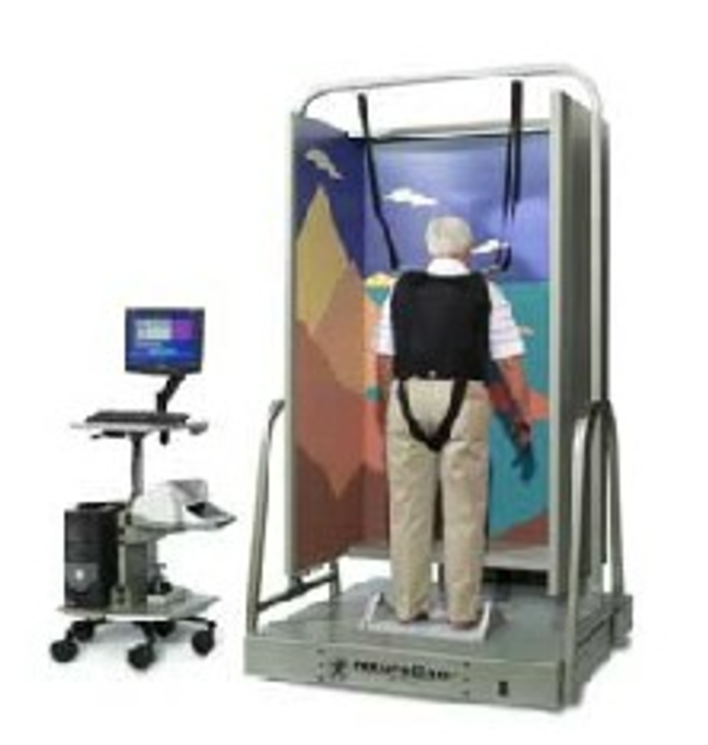
\includegraphics[height=5cm]{images/plateforme-posturographie.png}
    \caption{Plateforme posturographique}\label{fig:plateforme_posturographie}
  \end{subfigure}
  \begin{subfigure}[b]{0.45\textwidth}
    \centering
    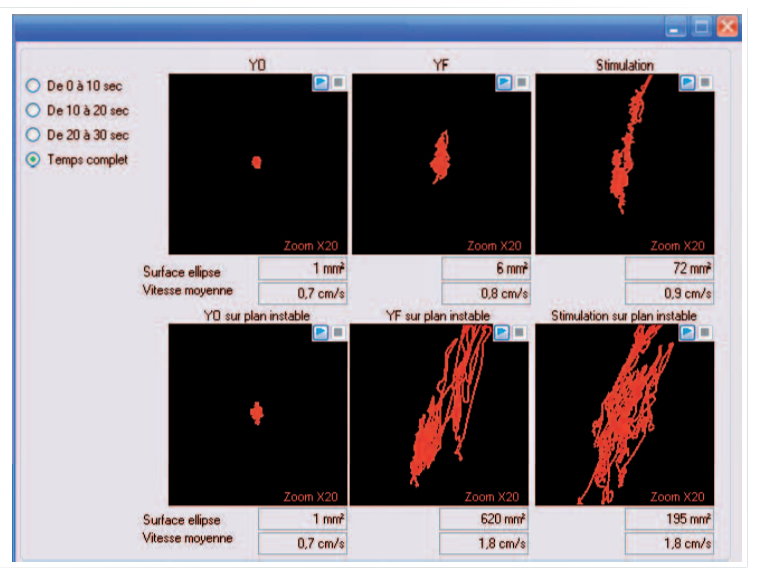
\includegraphics[height=5cm, width=\textwidth]{images/logiciel-analyse-posturographique.png}
    \caption{Logiciel d'analyse posturographique}\label{fig:logiciel_analyse_posturographique}
  \end{subfigure}
  \caption{Exemple de matériel utilisé dans le cadre d'analyse posturograpgique}\label{fig:exemple_posturographie}
\end{figure}

\subsection{Systèmes de baropodométrie}
Les dispositifs de baropodométrie évaluent les contraintes plantaires en employant des détecteurs de tension disposés sur une surface (plateformes) ou incorporés dans des semelles. 
Ces détecteurs enregistrent la distribution des forces sous les pieds et déterminent les points de tension supérieurs et inférieursD.

On utilise ces dispositifs pour examiner la dynamique et la statique du pied, principalement en podologie, orthopédie et rééducation. 
Ils servent à établir le diagnostic de maladies telles que les troubles posturaux ou les troubles du pied (comme la fasciite plantaire). 
Dans le domaine du sport, ils contribuent à perfectionner les compétences en course ou en marche.

\subsubsection{Exemples :}
\begin{itemize}
  \item \href{https://www.tekscan.com/products-solutions/systems/f-scan-system}{\textbf{Tekscan F-Scan}}
  \item \href{https://moticon.de/}{\textbf{Moticon OpenGo}}
\end{itemize}

\begin{figure}[ht]
  \centering
  \begin{subfigure}[b]{0.45\textwidth}
    \centering
    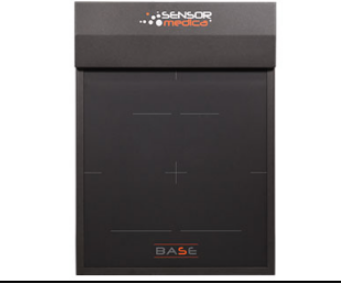
\includegraphics[height=5cm]{images/appareil-baropodometrie.png}
    \caption{Appareil de mesure de baropodométrie}\label{fig:appareil_baropodometrie}
  \end{subfigure}
  \begin{subfigure}[b]{0.45\textwidth}
    \centering
    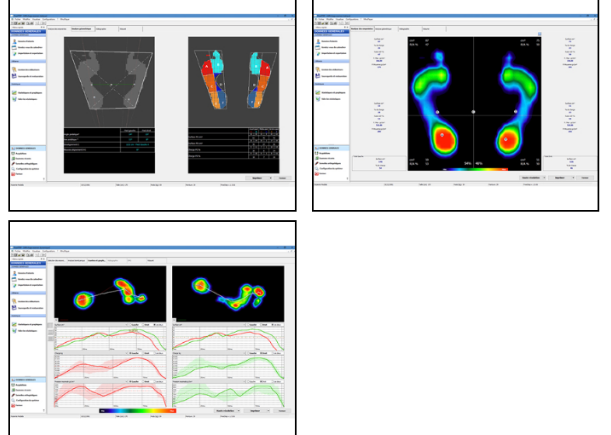
\includegraphics[height=5cm, width=\textwidth]{images/logiciel-analyse-baropodometrie.png}
    \caption{Logiciel d'analyse de baropodométrie}\label{fig:analyse_baropodometrie}
  \end{subfigure}
  \caption{Exemple de dispositifs de baropodométrie}\label{fig:exemple_baropodométrie}
\end{figure}

\subsection{Appareils d’électromyographie (EMG)}

Les dispositifs d'électromyographie consignent l'activité électrique produite par les muscles pendant leur contraction. 
Des électrodes de surface, installées sur la peau au-dessus du muscle, ou des électrodes intramusculaires, introduites directement dans le muscle, captent ces signaux. 
Les informations recueillies indiquent l'intensité, la prolongation et la fréquence de l'activation musculaire. 
Par la suite, ces signaux sont amplifiés et filtrés afin d'être examinés.

On utilise les instruments EMG pour examiner les associations musculaires et détecter les déséquilibres ou anomalies neuromusculaires. 
Ils servent à diagnostiquer des troubles comme les neuropathies ou les dystrophies musculaires en milieux hospitaliers. 
Dans le domaine sportif, l'EMG contribue à améliorer la performance musculaire et à empêcher les blessures. 
En conclusion, dans le processus de rééducation, ils surveillent les avancées des patients en évaluant la performance des exercices de renforcement.

\subsubsection{Exemples :}
\begin{itemize}
  \item \textbf{Noraxon Ultium EMG }
  \item \textbf{Delsys Trigno Wireless EMG }
  \item \textbf{BTS FREEEMG }
\end{itemize}

\begin{figure}[ht]
  \centering
  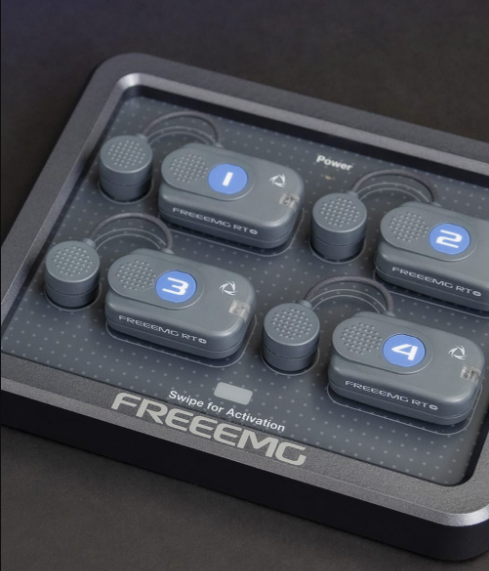
\includegraphics[height=5cm]{images/electrodes.png}
  \caption{Électrodes pour mesurer l'électromyographie}\label{fig:electrodes}
\end{figure}

\subsection{Pistes de marche électroniques}

Les pistes électroniques de marche sont des tapis munis de capteurs incorporés qui consignent les forces et la pression exercées au cours du mouvement.
Des paramètres tels que la vitesse de marche, la longueur du pas, le rythme et la symétrie font partie des informations collectées. 
Ces tapis peuvent aussi être associés à des dispositifs d'analyse vidéo ou des plateformes de force pour une analyse plus exhaustive.

Utilisées dans les laboratoires et les cliniques, ces pistes permettent d'évaluer les troubles de la marche et de suivre l'évolution des patients en réhabilitation. 
En recherche, elles offrent des données précises sur les performances locomotrices. 
Ces dispositifs sont également employés pour l'analyse des mouvements athlétiques dans le domaine du sport.

\subsubsection{Exemples :}
\begin{itemize}
  \item \href{https://www.gaitrite.com/}{\textbf{GAITRite Walkway}}
  \item \href{https://www.treadmetrix.com/}{\textbf{Treadmetrix System}}
\end{itemize}

\href{https://www.gaitrite.com/}{Voici un exemple de ce type de tapis de marche}

\subsection{Systèmes d’analyse vidéo du mouvement}

Ces dispositifs se servent de caméras (généralement infrarouges) et d'indicateurs positionnés sur les segments du corps afin d'enregistrer les mouvements dans en 2D ou 3D. 
L'analyse des trajectoires, des angles articulaires et des vitesses segmentaires est possible grâce aux informations recueillies. 
Des algorithmes d'intelligence artificielle sont également employés par certains systèmes contemporains pour réaliser des analyses sans marqueurs.

Dans le domaine de la recherche, ces dispositifs sont cruciaux pour examiner la cinématique globale du mouvement, comme c'est le cas dans les recherches biomécaniques ou les simulations sportives. 
En milieu hospitalier, ils contribuent au diagnostic des problèmes moteurs ou à la mesure de la performance fonctionnelle suite à une réhabilitation. 
Dans le domaine sportif, ils contribuent à perfectionner les méthodes des sportifs en offrant une analyse exacte de leurs mouvements.

\subsubsection{Exemples :}
\begin{itemize}
  \item \href{https://www.vicon.com/}{\textbf{Vicon Motion Systems}}
  \item \href{https://optitrack.com/}{\textbf{OptiTrack Motion Capture}}
  \item \href{https://www.qualisys.com/}{\textbf{Qualisys Motion Capture}}
\end{itemize}
Voir la vidéo : \href{https://www.youtube.com/watch?v=MTi32qJB_vo}{Laboratoire d'analyse du mouvement en 3D}